\chapter{The Knowledge Pyramid}
\begin{figure}[t]
    \centering
    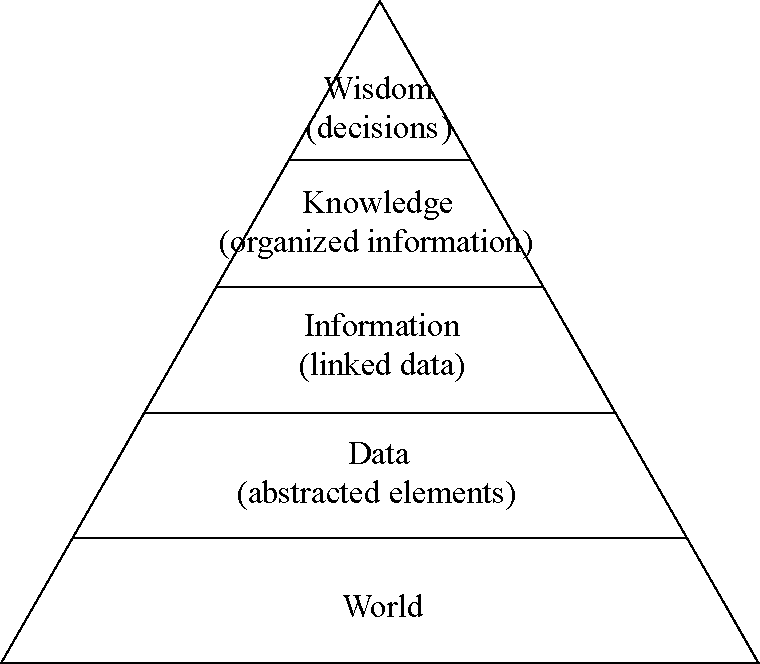
\includegraphics[scale=.7]{global/DIKW.pdf}
    \caption{The ``knowledge pyramid'' (also known as the ``Data Information Knowledge Wisdom pyramid'' or ``knowledge hierarchy''; adapted from \cite{DBLP:journals/oir/Stuart15b}).}
    \label{fig:dikw}
\end{figure}

Data science extracts actionable insights from raw data \cite{kelleher2018data}. The data transformation process is usually abstracted in the ``knowledge pyramid'' (also known as the ``Data Information Knowledge Wisdom pyramid'' or ``knowledge hierarchy''; \Cref{fig:dikw}), where data (i.e., symbols) are collected through measurements taken from the real world; information is processed and linked data that it is meaningful to scientists; knowledge is interpreted, understood, and organized information; and wisdom is knowledge in action. Climbing the pyramid is not a straightforward path and requires the iterative exploration and preparation of data so that patterns can be extracted, evaluated, and later deployed into models supporting effective decisions. 

Analytic applications strive to extract knowledge from data fueled by pervasive systems \cite{8423172}, where any device can be turned into a sensor leading to a huge volume and variety of available data \cite{vitali2021crop}. These \textit{unconventional}\footnote{We consider \textit{conventional} the data collected by operational databases, ERP (enterprise resource planning), and CRM (customer relationship management) enterprise systems} data (i.e., unstructured and non-relational data) have impacted on business intelligence (BI)---the discipline providing strategies and technologies to transform data into decision-making information---leading to BI 2.0, where decisions are drawn \textit{not only} on the data owned by the organization. Indeed, bigger data volumes lead to a holistic view of historic and current trends; higher data velocities ground decisions in continuously updated data, and broader data varieties provide many nuances of the matter at hand \cite{IBM4V}. On the one hand, volume and variety hinder the management, the integration, and the analysis of the collected data (from ``World'' to ``Data'' in \Cref{fig:dikw}), since each instance of unstructured data might have a different structure. This requires ad-hoc techniques for different data types (e.g., social networks \cite{DBLP:journals/snam/FranciaGG19} or sensor data \cite{DBLP:conf/mipro/FranciaGV19}). On the other hand, high availability has attracted scientists with no expertise in computer science or data engineering, requiring novel paradigms to support the ``Data''-to-``Knowledge''
%\footnote{Since ``wisdom'' is related to the \textit{application} of knowledge \cite{8423172}---besides no strict definition is given in the literature---we address the transformation of raw data into knowledge (i.e., patterns extracted with mining/machine learning models).} 
transformation with a higher abstraction level than formal programming languages (e.g., through graphical metaphors, recommender systems, or automatic transformation pipelines). Additionally, availability has enabled pervasive analyses, allowing data scientists to access data in hand-free contexts involving augmented reality and smart assistants.

While investigating these challenges, this thesis evolves into two parts.

\begin{figure}[t]
    \centering
    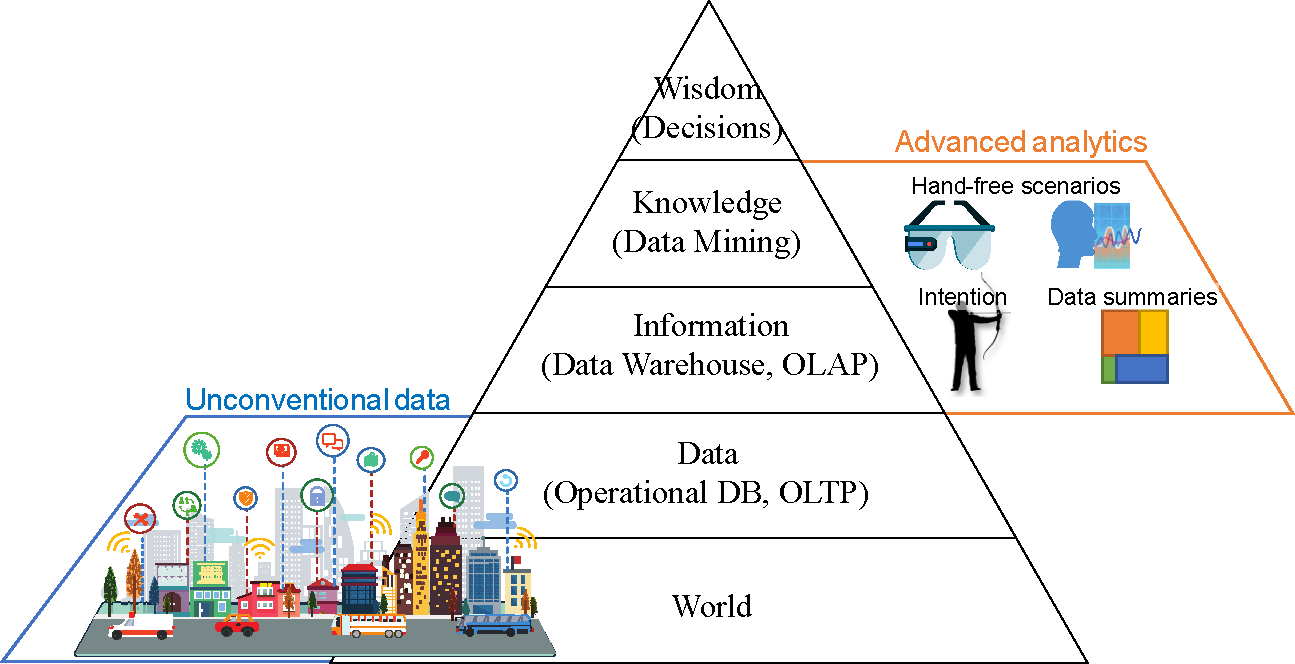
\includegraphics[scale=.65]{global/augmenting.pdf}
    \caption{Augmenting the knowledge pyramid with unconventional data (left) and advanced analytics (right).}
    \label{fig:aug}
\end{figure}

\paragraph{\Cref{part:trajectory}: Unconventional Data.}
Sensing provides real-time data upon which ``contextual'' decisions---ranging from user-centric to societal problems---are based. This includes data collected from human and technological assets (e.g., sensor or mobile networks), which are analyzed to monitor and manage urban and rural areas. Sensor data are highly available due to the growth of Internet of Things devices, have variable content, and their value comes from historic trends that range from hours to years \cite{kelleher2018data}. Such volume and variety demand for augmenting the knowledge pyramid with novel and scalable techniques for different data types (\Cref{fig:aug}). In urban mobility, spatiotemporal data (i.e., temporal sequences of spatial locations traced by moving objects and sampled through global or relative positioning sensors) are collected and processed for the sake of traffic analysis and forecasting, clustering of objects moving in similar paths, and habits profiling. Spatiotemporal data are challenging because of their uncertain, sparse, and multiresolution nature \cite{DBLP:journals/cacm/GilPBBBBCEGHHHK19}. Also, due to the number of moving objects (e.g., mobile devices, cars, taxis, and public transport in a metropolitan area) and to the sampling rate of positioning sensors (e.g., from minutes to seconds), mining mobility data easily scale up to big-data problems that require big-data solutions, hence introducing %a 
new business opportunities
% to analyze and extract information from data 
that were previously ignored because of technology limitations. Besides the valuable knowledge, due to high uniqueness \cite{DeMontjoye2013} and sensitivity (e.g., home and work locations), trajectory data expose individuals to privacy violations, demanding for ad-hoc techniques to (de-)anonymize historical trajectory datasets. In this direction, \Cref{part:trajectory} focuses on trajectory data and on the privacy implications of the publication of long-term mobility datasets.

\paragraph{\Cref{part:olap}: Advanced Analytics.}
Since the introduction of the relational model in the '70s, users used relational queries (e.g., SQL queries) to retrieve data collected in operational databases. This requires a good comprehension of programming languages and database management systems. Later, more user-friendly abstractions and tools provided a simpler view of the data, hiding the complexity of the underlying databases \cite{DBLP:journals/is/VassiliadisMR19} and transitioning from static (repetitive) workloads involving a few records (On-Line Transaction Processing, OLTP) to dynamic workloads (On-Line Analytical Processing, OLAP, and On-Line Analytical Mining, OLAM) involving a huge amount of records (\Cref{fig:aug}). The spread of data and analytical tools at hand has brought an increasing participation of data scientists with high competence in the business domain but low competence in computer science and data engineering \cite{DBLP:journals/is/VassiliadisMR19}. Indeed, data science emerged as an amalgamation of domain expertise with disciplines such as statistics, data mining, and databases \cite{vanderAalst2016}. Such amalgamation has brought challenges not only concerning big data volumes but also in terms of the increasing complexity and interdisciplinarity of the analytic questions. Enabling an effective participation in data science requires the investigation of user-centric paradigms supporting analytical querying and making knowledge extraction more accessible. Data scientists can benefit from proactive systems that ``understand'' the tasks at hand, make recommendations, and generate effective visualizations \cite{DBLP:journals/cacm/GilPBBBBCEGHHHK19}. For instance, in the digital twin scenario \cite{tao2018digital} where physical entities are mapped into a digital world, the synergy of personal assistants and augmented reality lacks analytic capabilities. Additionally, limited attention has been devoted to providing analytical reports that can be useful to let the user compare the current behavior of the visualized objects with their historical behavior. To this end, unconventional data sources, such as smart glasses and wearable devices, can be accessed by personal assistants (e.g., recommender systems) to address users' needs \cite{DBLP:conf/ictir/BahrainianC17}. Data scientists can interact with personal assistants through natural language interfaces which provide a higher abstraction level than formal queries and programming languages. In this direction, \Cref{part:olap} focuses on supporting data scientists with higher analytic abstractions than formal queries also in scenarios entailing pervasive data access. 